\section{Cluster-Matching-Based Method For Video Face Recognition}
\label{webmedia}

In this first work~\cite{mendes2020cluster}, we proposed a cluster-matching-based approach for video face recognition where clustering is used to group faces in both the face dataset and in the target video~(spatiotemporal localization).
%%
Consequently, classes do not have to be previously known, and the effort spent with annotations is significantly reduced --- as it is done over clusters instead of single images.
%%
Face recognition becomes a task of comparing clusters from the dataset with the ones extracted from images or video sources.
%%
Therefore, our approach is easily scalable and can be used to automatically generate video metadata. 

\subsection{Method}
\label{webmedia_method}

Our method intends to recognize people in video using CNNs and clustering algorithms.
%%
For didactic purposes we decided to divide our exposition in two phases: (i)~\emph{labeled clusters generation phase} and (ii)~\emph{cluster matching for video face recognition}, which are described in Sections~\ref{subsec:labeled_clusters} and \ref{subsec:cluster_match} respectively.

\subsubsection{Labeled Clusters Generation}
\label{subsec:labeled_clusters}

\begin{figure*}[!ht]
    \centering
    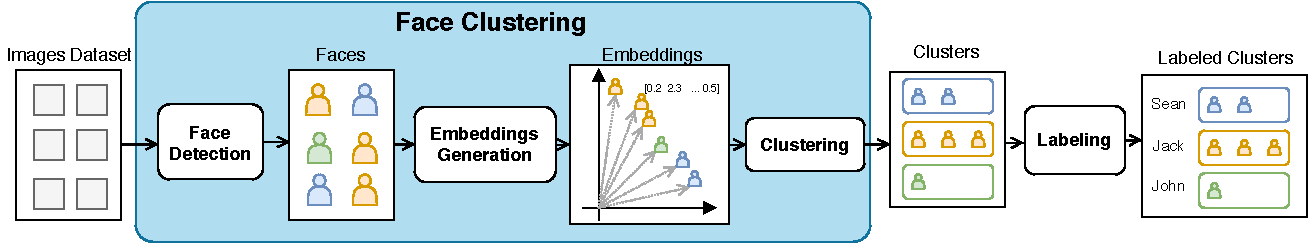
\includegraphics[width=\textwidth]{img/webmedia/labeled_clusters.pdf}
    \caption{Labeled clusters process.}
    \label{fig:labeled_clusters}
\end{figure*}

The \textit{Face Detection} step uses an object detection model for detecting faces in each of its images.
%%
This model is responsible for returning the bounding boxes of the faces present in the image, specified by the $x$ and $y$ axes coordinates of the upper-left corner and of the lower-right corner of the rectangle that establishes the visual limits that encapsulate each face. 
%%
With these bounding boxes, we can isolate and extract the bounded images, obtaining a dataset composed of images of faces only.


The objective of the \textit{Embeddings Generation} step is to represent each face image as a vector space in $\mathbb{R}^{n}$.
%%
To achieve that, it processes each of the faces generated in the previous step through a CNN, generating embeddings. 
%%
An embedding is a representation of the input in a lower dimensionality space.

In the \textit{Clustering} step, we group embeddings and, consequently, faces that are close in the embedding space using a clustering algorithm. 
%%
The clustering process should produce a partition of the dataset, i.e., each generated cluster represents a specific person, and the union of all clusters covers the whole dataset.

Finally, in the \textit{Labeling} step, we assign labels~(identities) to represent the clusters.
%%
Using this pipeline, instead of having to label every single face for constructing a labeled dataset, it is only necessary to label each generated cluster.
%%
Consequently, all the faces present in a cluster are assigned to the same label.
%%
At the end of this step, we have a dataset of labeled clusters.

\subsubsection{Cluster Matching for Video Face Recognition}
\label{subsec:cluster_match}

\begin{figure*}[!ht]
    \centering
    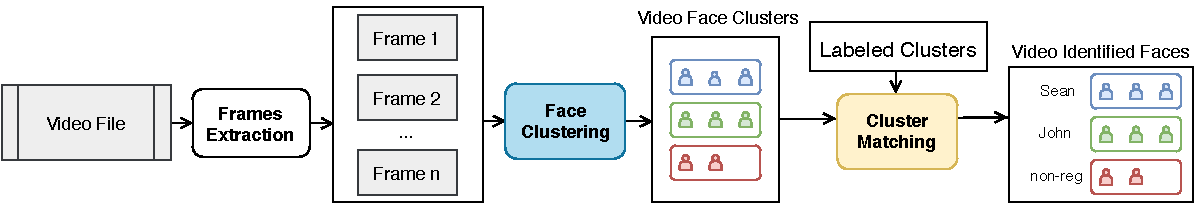
\includegraphics[width=\textwidth]{img/webmedia/video_face_recognition.pdf}
    \caption{Cluster-matching based method for automatic face recognition in video files.}
    \label{fig:cluster_matching}
\end{figure*}

This phase aims at recognizing the faces present in a video file. 
%%
It is divided in three steps: \emph{frames extraction}, \emph{face clustering} and \emph{cluster-matching}.
%%
Figure \ref{fig:cluster_matching} shows the pipeline we propose for this phase, described in the remainder of this subsection.

First, we perform \textit{Frames Extraction} by receiving a video file as input and extracting its frames according to a given frame rate. 
%%
These frames are used as a set of images for the next step.

Next, the \textit{Face Clustering} step, which is a macro-step that comprises the three first steps of the \emph{Labeled Clusters Generation} phase~(\emph{Face Detection}, \emph{Embeddings Generation}, and \emph{Clustering}), receives this set of images and returns a set of clusters of the faces present in the images received  (see Figure \ref{fig:labeled_clusters}).
%%
%In this phase, the input images are the frames of the video being processed.
%%
It is important to notice that this phase uses the same methods used for \emph{Labeled Clusters Generation}.
%%
Consequently, the embeddings of the faces from the video are part of the same embedding space as the data points (faces) in the labeled clusters.

Finally, the \textit{Cluster Matching} step receives the set of clusters from the video and the set of labeled clusters, which is used as a reference for recognizing the clusters (and consequently the faces) in the video.
%%
%%
We designed a method based on cluster distance for performing this recognition.

\subsection{Evaluation}

We have performed two experiments to evaluate our method. 
%%
The first evaluation aimed at measuring how well our approach of \emph{Face Clustering} performed using different combinations of CNNs and Clustering Algorithms. 
%%
The second evaluation aimed at measuring how well our approach performed on video. Each of these evaluations are describe in the following subsections.

\subsubsection{Faces Clustering Evaluation}
\label{faces_clustering_evaluation}
In the \emph{Face Detection} step, we use MTCNN~\cite{mtcnn} (Multitask
Cascaded Convolutional Networks) which is widely used for the face detection task.
%%
For the \emph{Embeddings Generation} step, we have three candidate CNNs that were previously trained on the VGGFace2 dataset~\cite{cao2018vggface2}. The three candidate CNNs used are VGG-16~\cite{vgg16}, ResNet-50~\cite{resnet} and SeNet-50~\cite{senet}. 
%%
For the \emph{Clustering} step, we selected the following clustering algorithms as candidates: k-Means~\cite{lloyd1982least}, affinity propagation~\cite{frey2007clustering}, and agglomerative clustering~\cite{ward1963hierarchical}.

We evaluate the models using the V-Measure~\cite{vmeasure}, which is an entropy-based measure that computes how successfully the criteria of homogeneity and completeness have been satisfied. This metric is extensively used for comparing clustering solutions and has been used in different domain fields such as biology~\cite{bio1}, computational linguistics~\cite{nlp1}, and document engineering~\cite{doceng}.
%%
The homogeneity score is perfect when a clustering algorithm assigns only those data points that are members of a single class to a single cluster, so that the entropy is zero in each cluster. The Completeness score is symmetrical with respect to homogeneity, and it is perfect when a clustering assigns all data points that are members of the same class to a single cluster.

Table \ref{tab:results_clustering} shows the homogeneity, completeness, and V-Measure for each combination of CNN and clustering algorithm.
%%
From this table, one can conclude that the best combination of CNN and clustering algorithm was SeNet-50 with Agglomerative Clustering.
%%
For this reason, we decided to use SeNet-50 for the \emph{Embeddings Generation} phase and the Agglomerative Clustering algorithm for the \emph{Clustering} phase.


\begin{table}[!ht]
\small
\centering
\caption{Results of the evaluation of the clusters created by each combination of CNN and clustering algorithms.}
\begin{tabular}{@{}ccccc@{}}
\toprule
\textbf{CNN} & \textbf{Clustering} & \textbf{$h$} & \textbf{$c$} & \textbf{$V_1$} \\ \midrule
                  & KM                  & 0.9665                     & 0.9675                      & 0.9670             \\
ResNet-50         & AP                  & 0.0000                     & 1.0000                      & 0.0000             \\
                  & AC                  & 0.9821                     & 0.9798                      & 0.9810             \\ \midrule
                  & KM                  & 0.9725                     & 0.9726                      & 0.9725             \\
SeNet-50          & AP                  & 0.9859                     & 0.9558                      & 0.9706             \\
                  & \textbf{AC}         & \textbf{0.9862}            & \textbf{0.9833}             & \textbf{0.9847}    \\ \midrule
                  & KM                  & 0.8340                     & 0.8415                      & 0.8378             \\
VGG-16            & AP                  & 0.0000                     & 1.0000                      & 0.0000             \\
                  & AC                  & 0.8899                     & 0.8929                      & 0.8914             \\
\end{tabular}
\label{tab:results_clustering}
\vspace{-1em}
\end{table}


\subsubsection{Video Face Recognition Evaluation}

To evaluate our complete pipeline, we selected videos that contain only registered people (videos \emph{a} to \emph{d}), videos with both registered and non-registered people (videos \emph{e} to \emph{i}) and videos with only non-registered people (videos \emph{j} to \emph{m}).

For performing the face identification on a video file, we first extract its frames using a frame rate of 1fps.
%%
For each of the frames, we extract the faces present on it using MTCNN~\cite{mtcnn}. 
%%
Then, for each face identified, we resize it to 224x244, extract its embedding using SeNet-50 and cluster these faces using the Agglomerative Clustering algorithm.

Next, we perform the \emph{Cluster Matching} with the labeled clusters and the video face clusters.
%%
At the end of this process, each face present on the video is labeled either with the name of a registered person or as non-registered.

%%
We evaluate our method by the Precision~(Prec), Recall (Rec), and F1-Score for the faces in the video. 
%%
As usual, the Precision is defined as the percentage of detected faces that our method correctly labels, 
%%
the Recall gives the percentage of faces that our method correctly labels among all faces in the video, and 
%%
the F1-score represents an overall performance metric based on the  harmonic mean of the precision and recall.
\begin{table}[!ht]
\centering
\small
\caption{Results using the proposed approach in videos.}
\vspace{-1em}
\label{tab:results_videos}
\begin{tabular}{@{}cccccccc@{}}
\toprule
\textbf{Video} & \textbf{\#P} & \textbf{\#R} & \textbf{\#F} & \textbf{\#EM} & \textbf{Rec.} & \textbf{Prec.} & \textbf{F1} \\ 
\multicolumn{8}{c}{\cellcolor[HTML]{C0C0C0}{\color[HTML]{000000} videos with only registered people}}\\
a%\footnote{https://youtu.be/QjTZ\_TE1U\_g} 
& 1 & 1  & 105 & 105 & 100.000\% & 100.000\% & 100.000\%  \\
b%\footnote{https://youtu.be/4D5GGR3g\_7c}
& 1 & 1  & 80  & 79  & 100.000\% & 98.765\%  & 99.379\%   \\
c%\footnote{https://youtu.be/quYNTUsOTb8}
& 1 & 1 & 60  & 59   & 100.000\% &	98.113\% & 99.048\%   \\
d%\footnote{https://youtu.be/eB6kJYaoxHc}
& 2 & 2  & 226 & 226 & 100.000\% & 100.000\% & 100.000\%  \\ 
\multicolumn{8}{c}{\cellcolor[HTML]{C0C0C0}{\color[HTML]{000000} videos with both registered and non-registered people}}\\
e%\footnote{https://youtu.be/j07yExfJ4mA}
& 2 & 1  & 101 & 99  & 100.000\% & 98.113\%  & 99.048\%   \\
f%\footnote{https://youtu.be/Db2I1uUyDlE}
& 2 & 1  & 650 & 650 & 100.000\% & 100.000\% & 100.000\%  \\
g%\footnote{https://youtu.be/sf56sWeiMyo}
& 8 & 1  & 201 & 190 & 96.471\%  & 96.850\%  & 96.660\%   \\
h%\footnote{http://youtu.be/dYAFXogdqW4}
& 4 & 1  & 231 & 215 & 98.097\%  & 98.514\%  & 98.305\%   \\
i%\footnote{http://youtu.be/NHglWWOKmc4}
& 2 & 1  & 88  & 88  & 100.000\% & 100.000\% & 100.000\%  \\ 
\multicolumn{8}{c}{\cellcolor[HTML]{C0C0C0}{\color[HTML]{000000} videos with only non-registered people}}\\
j%\footnote{https://youtu.be/UH0nTHb6OdY}
& 6 & 0  & 625 & 617 & 99.551\%  & 99.551\%  & 99.551\%   \\
k%\footnote{http://youtu.be/wHN5vYlJ-Vk}
& 2 & 0  & 231 & 228 & 100.000\% & 98.872\%  & 99.433\%   \\
l%\footnote{http://youtu.be/WwRdjf4eEgk}
& 2 & 0  & 131 & 121 & 99.482\%  & 95.522\%  & 97.462\%   \\
m%\footnote{http://youtu.be/3dIVdsiPDH8}
& 1 & 0  & 225 & 222 & 99.556\%  & 99.115\%  & 99.335\%   \\
\bottomrule
\end{tabular}
\vspace{-1em}
\end{table}
We also count the number of exact frames match (\#EM). It corresponds to the number of frames (\#F) for which our method correctly labeled all the faces that appears. 
%%
Table \ref{tab:results_videos} shows the results we obtained, the number of different people in each video~(\emph{\#P}), and the number of people who are present in the labeled clusters~(\emph{\#R}).

One can observe that our method is able to correctly classify the faces of people that are present in the labeled clusters while also being able to tell when a person is not registered in the labeled clusters.
%%
Our method can also be used to generate metadata in video files indicating the people that appear in it.
%%
Figure \ref{fig:timeline_pol} shows the first 12 seconds of \emph{Video d}~(detailed in Table \ref{tab:results_videos}) where two identified Brazilian politicians are shown in each frame with its respective colored cluster.

\begin{figure}[!ht]
    \centering
    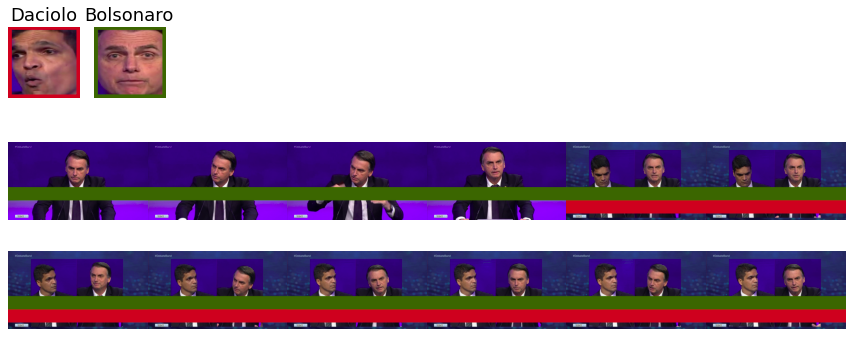
\includegraphics[width=0.6\linewidth]{img/webmedia/timeline_pol.png}
\vspace{-1em}
    \caption{Timeline with tagged frames by their clusters of registered people}
    \label{fig:timeline_pol}
\end{figure}

Besides being able to recognize people in video files, by using face embeddings and clustering, we can detect the frames where the same person appears without even knowing who the person is or if he/she is in the labeled clusters.
%%
This can be done by following the pipeline described in Figure \ref{fig:cluster_matching} up to the \emph{Face Clustering} step, obtaining the video face clusters.
%%
Figure \ref{fig:timeline} shows the first 24 seconds of \emph{Video j}~(detailed in Table \ref{tab:results_videos}) with the frames tagged with the clusters identified in each frame, where each color represents a cluster.

\begin{figure}[!ht]
    \centering
    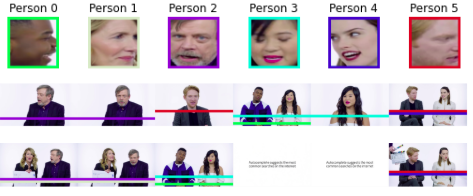
\includegraphics[width=0.6\linewidth]{img/webmedia/timeline2.png}
    \caption{Timeline with tagged frames by their clusters of non-registered people}
    \label{fig:timeline}
\end{figure}